
\documentclass[12pt, a4paper]{article}

\usepackage{graphicx}
\usepackage{xcolor}
\usepackage{float}
\usepackage{svg}
\usepackage[colorlinks=true, linkcolor=black, urlcolor=blue, citecolor=green]{hyperref}
\usepackage{enumitem}
\usepackage[italian]{babel}
\usepackage{lastpage}  % Pacchetto per ottenere il numero totale delle pagine
\usepackage{fancyhdr}  % Pacchetto per personalizzare l'intestazione e il piè di pagina
\usepackage[margin=1in]{geometry}
\usepackage{array}
\newcolumntype{C}[1]{>{\centering\arraybackslash}p{#1}}
\newcolumntype{L}[1]{>{\raggedright\arraybackslash}p{#1}}
\graphicspath{ {images/} {../shared/images/} }
\definecolor{unipd}{HTML}{B5121B}

\addto\captionsitalian{\renewcommand{\contentsname}{Indice}}

\setcounter{secnumdepth}{5}
\setcounter{tocdepth}{5}
\makeatletter
\newcommand\subsubsubsection{\@startsection{paragraph}{4}{\z@}{-2.5ex\@plus -1ex \@minus -.25ex}{1.25ex \@plus .25ex}{\normalfont\normalsize\bfseries}}
\newcommand\subsubsubsubsection{\@startsection{subparagraph}{5}{\z@}{-2.5ex\@plus -1ex \@minus -.25ex}{1.25ex \@plus .25ex}{\normalfont\normalsize\bfseries}}
\makeatother

\pagestyle{fancy}% Imposta lo stile di pagina su "fancy"
\fancyhf{}% Cancella intestazioni e piè di pagina
\fancyfoot[C]{\thepage{} di \pageref{LastPage}} % Imposta il piè di pagina centrale come "numero pagina di totale pagine"
\renewcommand{\headrulewidth}{0pt} % Imposta la larghezza della linea di intestazione a 0 punti

%\newcommand{\data}{GG mese AAAA}
\newcommand{\titolo}{Specifica Tecnica}
%\newcommand{\responsabile}{Responsabile}
\newcommand{\verificatore}{
    Matteo Piron 
}
\newcommand{\redattore}{
    Derek Gusatto \\
    & Ion Bourosu \\
    & Alessandro Benin 
}
\newcommand{\uso}{Esterno}
\newcommand{\destinatari }{
   %& Vimar S.p.A.  \\
    & Tullio Vardanega  \\
    & Riccardo Cardin  }
\newcommand{\abstractcontent}{abstract ...}

\begin{document}

\begin{minipage}[]{0.3\textwidth}
\includesvg[width=\linewidth]{pebkac.svg} 
\end{minipage}
\hspace{0.1\textwidth}
\begin{minipage}[]{0.6\textwidth}
  {\Large \textbf{PEBKAC}} \\
  Email: \href{mailto:pebkacswe@gmail.com}{pebkacswe@gmail.com} \\
  Gruppo: 11
\end{minipage}

\bigskip

\begin{minipage}[]{0.3\textwidth}
\includesvg[width=\linewidth]{logo_unipd.svg} 
\end{minipage}
\hspace{0.1\textwidth}
\begin{minipage}[]{0.6\textwidth}
  \textcolor{unipd}{
    \textbf{Università degli Studi di Padova} \\
    Corso di Laurea: Informatica \\
    Corso: Ingegneria del Software \\
    Anno Accademico: 2024/2025
  }
\end{minipage}


\bigskip
\bigskip
\bigskip
\begin{center}
  \Huge\textbf{Verbale Interno}

  \Large\textbf{\data}
\end{center}

\bigskip


\begin{center}
\textbf{Informazioni sul documento}: \\
\vspace{0.5cm}

\begin{tabular}{r|l}
    \textbf{Responsabile} & Tommaso Zocche \\ 
    \textbf{Verificatore} & Alessandro Benin \\ 
    \textbf{Redattore} & Tommaso Zocche \\ 
    \textbf{Uso} & Interno \\ 
    \textbf{Destinatari} & Tullio Vardanega \\ & Riccardo Cardin \\ 
\end{tabular}

\vfill

\textbf{Abstract}: \\
\vspace{0.5cm}
L'obiettivo dell'incontro è stato definire l'ordine di preferenza dei capitolati a seguito degli incontri avuti con le aziende interessate e iniziare a redigere il prospetto orario del gruppo.
\end{center}


\bigskip
\newpage

\section*{Registro delle modifiche}
\begin{table}[H]
    \begin{tabular}{|c|c|c|c|p{5cm}|}
        \hline
         \textbf{Versione} &  \textbf{Data} &  \textbf{Autore} &  \textbf{Ruolo} & \textbf{Descrizione} \\
          \hline
          &  &  & Responsabile & Approvazione e rilascio\\
          \hline
          0.1.0 & 17/11/2024 & Alessandro Benin & Verificatore  & Verificato \\
          \hline
          0.0.1 & 13/11/2024 & Derek Gusatto & Amministratore  & Stesura iniziale \\
          \hline
    \end{tabular}
\end{table}
\newpage
\tableofcontents
\newpage
% VERBALE
% \section{Informazioni generali}
\begin{itemize}
  \item \textbf{Tipo riunione}: esterna
  \item \textbf{Luogo}: telematica, Teams
  \item \textbf{Data}: 25 novembre 2024
  \item \textbf{Ora inizio}: 16.00
  \item \textbf{Ora fine}: 17.00
  
  \item \textbf{Presenti}:
  \begin{itemize}
    \item Alessandro Benin
    \item Ion Bourosu
    \item Matteo Gerardin
    \item Derek Gusatto
    \item Davide Martinelli
    \item Matteo Piron
    \item Tommaso Zocche
    \item[$\star$] Mariano Sciacco (Vimar S.p.A.)
    \item[$\star$] Francesca Stival (Vimar S.p.A.)
  \end{itemize}

  \item \textbf{Assenti}:
 
\end{itemize}
% \newpage
% \section{Riassunto della riunione}
Nella presente riunione ci siamo allineati sugli ultimi task mancanti per la candidatura alla prima revisione RTB, che il gruppo si è impegnato a prensentare entro la fine della giornata. Risultano quindi mancanti:
\begin{itemize}
    \item La verifica del documento Norme di Progetto;
    \item L'aggiornamento del sito di presentazione ;
    \item La Lettera di Presentazione;
\end{itemize}

Viene quindi stilata dal gruppo la Lettera di Presentazione e il presente verbale.
% \newpage
% \section{Todo}
Durante la riunione sono emersi i seguenti task da svolgere.

\begin{center}
  \begin{tabular}{|p{5cm}|p{8cm}|}
    \hline
    \textbf{Assegnatario}       & \textbf{Task Todo} \\ \hline
     Derek Gusatto   &  Stesura Verbale Esterno 13/11/2024\\ \hline
     \textit{autoassegnazione}  & Condivisione del verbale e dei repo GitHub con Vimar S.p.A. \\ \hline
     \textit{autoassegnazione}  & Condivisione con Vimar S.p.A. dei nominativi e rispettive e-mail dei membri del gruppo \\ \hline
     Mariano Sciacco  & Invio invito riunione periodica per SAL \\ \hline
  \end{tabular}
\end{center}
\vspace{4cm}
\noindent Firma del referente Vimar S.p.A.: \underline{\hspace{5cm}}

%LISTA FIGURE
\listoffigures 
\newpage
%LISTA TABELLE
\listoftables
\newpage

\section{Introduzione}
Questo documento mira a garantire chiarezza e uniformità nella terminologia utilizzata all'interno della documentazione del progetto, riducendo al minimo le ambiguità o potenziali incomprensioni. A tal fine, include un glossario che fornisce definizioni precise per i termini specifici del dominio d'uso.
Per facilitare la consultazione, i termini sono organizzati in ordine alfabetico, consentendo una navigazione semplice e immediata. Inoltre, in tutti gli altri documenti del progetto, i termini presenti nel Glossario saranno identificati da un simbolo di riferimento, rappresentato da una "G" in pedice.
\newpage
\section{Tecnologie }
In questa sezione si espone una panoramica delle tecnologie adottate. Si ha la descrizione delle tecnologie e dei linguaggi di programmazione utilizzati, delle librerie\textsubscript{G} e dei framework\textsubscript{G} necessari, oltre che delle infrastrutture realizzate. 
\subsection{Docker}
Docker\textsubscript{G} è una piattaforma per la containerizzazione che consente di impacchettare, distribuire ed eseguire applicazioni in ambienti isolati e riproducibili. Il nostro progetto utilizza Docker per garantire una gestione efficiente delle dipendenze, facilitare il deployment e migliorare la portabilità del sistema su diverse infrastrutture.
L’uso di Docker permette di standardizzare l’ambiente di sviluppo e produzione, riducendo problemi di compatibilità tra sistemi operativi e versioni di software. I container definiti nel progetto includono il backend, il frontend e il database PostgreSQL, ciascuno configurato per garantire modularità e scalabilità. Rispetto ad altre alternative (e.g. Vagrant) Docker è stato scelto per la sua efficienza e facilità d'uso.
\subsubsection{Vantaggi}
\begin{itemize}
    \item \textbf{Isolamento e portabilità}: Ogni servizio è eseguito in un container indipendente, evitando conflitti tra dipendenze e facilitando il deployment su diverse piattaforme.
    \item \textbf{Scalabilità}: L’architettura a container permette di scalare orizzontalmente i servizi in base al carico di lavoro, migliorando le prestazioni del sistema.
    \item \textbf{Riproducibilità}: Grazie alla definizione di immagini Docker e file di configurazione YAML, l’ambiente di esecuzione può essere ricreato in modo identico su qualsiasi macchina.
    \item \textbf{Facilità di gestione e automazione}: L’integrazione con Docker Compose permette di avviare, arrestare e configurare l’intero sistema con un singolo comando, migliorando l’efficienza nella gestione dell’infrastruttura.
\end{itemize}
\subsubsection{Svantaggi}
\begin{itemize}
    \item \textbf{Consumo di risorse}: L’esecuzione di più container può richiedere un utilizzo elevato di CPU e memoria, specialmente in ambienti con risorse limitate.
    \item \textbf{Complessità nella configurazione}: La gestione della rete tra container, la persistenza dei dati e la sicurezza richiedono una configurazione attenta per evitare problemi di isolamento e performance.
    \item \textbf{Overhead nella virtualizzazione}: Sebbene più leggero rispetto alle macchine virtuali, Docker introduce un livello di astrazione che può impattare leggermente le prestazioni rispetto all’esecuzione nativa.
\end{itemize}
\subsection{Flask}
Flask\textsubscript{G} è un micro-framework web per Python, progettato per facilitare lo sviluppo di applicazioni web in modo semplice e veloce. Non richiede strumenti o librerie particolari per funzionare e non impone una struttura rigida al progetto. Abbiamo deciso di utilizzarlo per implementare un'API RESTful\textsubscript{G}, che segue i prinipi REST\textsubscript{G}, per gestire sessioni, conversazioni, messaggi e feedback, integrando anche funzionalità di intelligenza artificiale per generare risposte a domande attraverso un modello di linguaggio LLM\textsubscript{G} e un sistema di embedding\textsubscript{G}. Nel nostro sistema, Flask è la parte del back-end\textsubscript{G} che permette la connessione con un front-end\textsubscript{G} per la gestione delle interazioni con l'utente, grazie a un sistema di routing\textsubscript{G} che definisce delle rotte per gestire le richieste HTTP\textsubscript{G} (GET, POST, PUT e DELETE). 
\subsubsection{Vantaggi}
\begin{itemize}
    \item Non impone una struttura rigida, permettendo al team di sviluppo di organizzare il codice senza troppi vincoli e di integrare librerie strettamente necessarie;
    \item È semplice, quindi adatto a che si interfaccia per la prima volta allo sviluppo web con Python\textsubscript{G};
    \item L'integrazione con tecnologie avanzate come LLM\textsubscript{G} e sistemi di embedding\textsubscript{G}, dimostra la sua capacità di supportare soluzioni complesse.
\end{itemize}
\subsubsection{Svantaggi}
\begin{itemize}
    \item La flessibilità d'altro canto può risultare un rallentamento, essendo che manca la standardizzazione nel codice, specialmente in un contesto in cui il team è inesperto.
\end{itemize}

\subsection{Scrapy}
Scrapy\textsubscript{G} è un framework\textsubscript{G} open-source per Python\textsubscript{G} progettato specificamente per il web scraping\textsubscript{G}, ovvero l'estrazione di dati da siti web, nel nostro caso dal sito di Vimar. È basato su un'architettura asincrona\textsubscript{G}, che lo rende adatto per il crawling\textsubscript{G} di grandi volumi di dati. Per il nostro progetto abbiamo deciso di adottare un approccio che vede lo scraping come componente a sè stante. Dunque, l'inserimento dei dati avviene da un file JSON\textsubscript{G} dove sono stati caricati e aggiornati precedentemente.
\subsubsection{Vantaggi}
\begin{itemize}
    \item L'architettura asincrona ci permette di gestire un grande numero di richieste contemporaneamente;
    \item La seprazione fra la gestione delle richieste, l'elaborazione dei dati e il salvataggio dei risultati facilitano lo sviluppo e la manutenzione del codice;
    \item Permette di salvare i dati in formati diversi (JSON\textsubscript{G}, CSV\textsubscript{G} o XML\textsubscript{G}) e di integrarli facilmente con database o altre applicazioni.
\end{itemize}
\subsubsection{Svantaggi}
\begin{itemize}
    \item La scarsa esperienza nell'ambito del web scraping\textsubscript{G} può rallentare il processo, richiedendo più tempo per l'apprendimento di tale tecnologia;
    \item Si possono incotrare rallentamenti nel caso di politiche di crawling\textsubscript{G} specifiche o blocchi da parte dei siti web.
\end{itemize}

\subsection{Ollama}
Ollama\textsubscript{G} è una piattaforma leggera ed efficace per eseguire modelli di intelligenza artificiale in locale, con un'architettura ottimizzata che garantisce prestazioni elevate con un utilizzo ridotto di risorse. È più semplice e intuitiva rispetto ad LLM Studio, risultando ideale per il nostro progetto.
\subsubsection{Vantaggi}
\begin{itemize}
    \item Più leggero ed efficiente, consumando meno risorse e offrendo migliori prestazioni su hardware\textsubscript{G} standard;
    \item Interfaccia\textsubscript{G} più semplice e intuitiva, facile da usare, anche senza configurazioni complesse.
\end{itemize}
\subsubsection{Svantaggi}
\begin{itemize}
    \item Meno opzioni avanzate di personalizzazione per l'addestramento;
    \item Meno strumenti integrati per il monitoraggio e l'analisi delle prestazioni del modello.
\end{itemize}

\subsection{PostgreSQL}
PostgreSQL\textsubscript{G} è un sistema di gestione di database relazionale (RDBMS) open-source che garantisce elevate prestazioni, affidabilità e scalabilità. È stato scelto per il nostro progetto in quanto offre una gestione avanzata degli indici e la possibilità di estendere le sue funzionalità tramite moduli aggiuntivi. PostgreSQL supporta inoltre l’archiviazione e la gestione di dati non strutturati grazie a tipi di dati avanzati come JSONB e l’estensione VECTOR\textsubscript{G}, fondamentale per l’elaborazione di dati ad alta dimensionalità, come gli embedding generati da modelli di intelligenza artificiale.
\subsubsection{Vantaggi}
\begin{itemize}
    \item \textbf{Affidabilità e consistenza}: PostgreSQL garantisce la conformità agli standard ACID (Atomicità, Consistenza, Isolamento, Durabilità), assicurando l’integrità dei dati anche in presenza di errori o interruzioni del sistema;
    \item \textbf{Supporto per estensioni avanzate}: PostgreSQL può essere esteso con moduli come PostGIS (per dati geografici) e pgvector, che consente di memorizzare e gestire vettori ad alta dimensionalità, rendendolo adatto all’integrazione con sistemi di ricerca semantica e modelli di intelligenza artificiale;
    \item \textbf{Ottimizzazione delle query}: Il motore di PostgreSQL utilizza un planner sofisticato in grado di ottimizzare le query grazie all’uso di indici B-Tree, GIN, GiST e BRIN, migliorando le prestazioni nelle operazioni di ricerca e aggregazione;
    \item \textbf{Scalabilità e parallelismo}: Supporta replica sincrona e asincrona, partizionamento delle tabelle e parallelizzazione delle query, garantendo elevate prestazioni in ambienti distribuiti e con grandi volumi di dati.
\end{itemize}
\subsubsection{Svantaggi}
\begin{itemize}
    \item \textbf{Maggiore complessità di gestione}: Rispetto ad altri RDBMS, PostgreSQL richiede una configurazione più avanzata per ottenere prestazioni ottimali, in particolare nella gestione degli indici e della cache;
    \item \textbf{Consumo di risorse}: Le operazioni di scrittura e indicizzazione possono risultare più costose in termini di memoria e CPU rispetto ad alternative come MySQL o SQLite, specialmente per applicazioni con carichi di lavoro elevati.
\end{itemize}

\subsection{Angular}
Angular\textsubscript{G} è un framework open-source per lo sviluppo di applicazioni web single-page (SPA\textsubscript{G}). È basato su TypeScript\textsubscript{G}, un superset di JavaScript\textsubscript{G}. Nel nostro sistema è utilizzato per il front-end\textsubscript{G}, permettendo una gestione efficiente delle interazioni utente e una comunicazione fluida con il back-end\textsubscript{G} tramite API RESTful\textsubscript{G}. Si tratta di una comunicazione asincrona\textsubscript{G} (di default), grazie all'uso di RxJS\textsubscript{G} e degli Observables\textsubscript{G}. Quest'approccio sfrutta il pattern reattivo\textsubscript{G} per gestire le oprazioni come le richieste HTTP\textsubscript{G}. 
\subsubsection{Vantaggi}
\begin{itemize}
    \item Utilizza un sistema di moduli e componenti che favorisce il riciclo del codice e una struttura organizzata;
    \item Si basa sul two-way of data binding\textsubscript{G}, ovvero la sincronizzazione automatica dei dati tra modello\textsubscript{G} e vista\textsubscript{G};
    \item Grazie all'utilizzo di Angular CLI\textsubscript{G} alcune attività come la creazione del progetto e la generazione delle componenti, vengono automatizzate;
    \item Si integra facilmente con il back-end tramite sevizi HTTP, redendolo un'ottima scelta per applicazioni che richiedono una comunicazione costante con il server.
\end{itemize}
\subsubsection{Svantaggi}
\begin{itemize}
    \item Richiede molto tempo per l'apprendimento a causa della sua complessità e della necessità di imparare concetti come moduli, servizi e dependency injection\textsubscript{G};
    \item Le app sviluppate con Angular possono richiedere molto spazio;
    \item Il ciclo di aggiornamente è molto frequente perciò è possibile che ci sia la necessità di intervenire per mantenrlo compatibile alle nuove versioni.
\end{itemize}

\subsection{Linguaggi e formato dati}
\subsubsection{Python}

\subsubsection{SQL}
SQL (Structured Query Language)\textsubscript{G} è il linguaggio utilizzato per la gestione e manipolazione dei dati in PostgreSQL. Il nostro progetto sfrutta SQL per la definizione dello schema del database, la gestione delle relazioni tra le entità e l’esecuzione di operazioni di lettura, scrittura, aggiornamento ed eliminazione dei dati. Abbiamo scelto SQL\textsubscript{G} rispetto a NoSQL\textsubscript{G} perché garantisce affidabilità, coerenza e query avanzate, fondamentali per il nostro progetto.
\subsubsection{Vantaggi}
\begin{itemize}
    \item Strutturato e organizzato, Ideale per dati relazionali con schemi ben definiti;
    \item Query\textsubscript{G} potenti e precise, grazie a JOIN\textsubscript{G}, filtri e funzioni avanzate;
    \item Ampio supporto, Usato in molti database\textsubscript{G}.
    \item L’integrazione con pgvector permette di eseguire operazioni di similarità su dati rappresentati come vettori, abilitando funzionalità di nearest neighbor search per applicazioni di machine learning e retrieval aumentato.
\end{itemize}
\subsubsection{Svantaggi}
\begin{itemize}
    \item Meno flessibile con dati non strutturati, NoSQL\textsubscript{G} è più adatto per dati dinamici e documentali;
    \item Scalabilità orizzontale complessa, NoSQL\textsubscript{G} può essere più efficiente per sistemi distribuiti su larga scala;
    \item Rigidità nella modifica dello schema, cambiare la struttura del database\textsubscript{G} può essere complicato in ambienti SQL\textsubscript{G}.
\end{itemize}

\subsubsection{YAML}
YAML (YAML Ain’t Markup Language)\textsubscript{G} è un formato di serializzazione dati leggibile dall’uomo, utilizzato principalmente per configurazioni e automazione, come nei file Docker Compose\textsubscript{G}. La sua sintassi basata sull’indentazione lo rende più leggibile rispetto ad altri formati, ma richiede attenzione alla formattazione.
\subsubsection{Vantaggi}
\begin{itemize}
    \item Maggiore leggibilità grazie alla sintassi senza parentesi e virgolette;
    \item Supporta commenti, facilitando la documentazione delle configurazioni;
    \item Permette riferimenti e ancoraggi per riutilizzare parti del file\textsubscript{G}.
\end{itemize}
\subsubsection{Svantaggi}
\begin{itemize}
    \item Sensibile all’indentazione, aumentando il rischio di errori difficili da individuare;
    \item Parsing\textsubscript{G} più lento rispetto ad altri formati come JSON\textsubscript{G};
    \item Meno diffuso per l’interscambio dati rispetto ad altri standard.
\end{itemize}

\subsubsection{JSON}
JSON\textsubscript{G} è un formato leggero per lo scambio di dati tra applicazioni, ampiamente utilizzato nelle API\textsubscript{G} e nella comunicazione tra servizi. La sua sintassi basata su coppie chiave-valore e array\textsubscript{G} lo rende facile da elaborare e compatibile con la maggior parte dei linguaggi di programmazione.
\begin{itemize}
    \item Struttura semplice e facilmente interpretabile da macchine e sviluppatori;
    \item Parsing\textsubscript{G} più lento rispetto ad altri formati come JSON;
    \item Standard per lo scambio di dati tra sistemi diversi.
\end{itemize}
\subsubsection{Svantaggi}
\begin{itemize}
    \item Meno leggibile rispetto a YAML\textsubscript{G}, specialmente in configurazioni complesse;
    \item Non supporta commenti, rendendo più difficile documentare il codice;
    \item Più rigido nella sintassi, con obbligo di virgolette e parentesi.
\end{itemize}
\newpage
\section{Architettura di sistema }
\subsection{Modello Architetturale}
Il progetto Vimar GENIALE rappresenta un’applicazione moderna e avanzata per la gestione di conversazioni intelligenti, sviluppata con un’architettura distribuita e tecnologie all’avanguardia. La sua struttura è pensata per garantire flessibilità, scalabilità e manutenibilità nel tempo, integrando diversi componenti che collaborano per offrire un’esperienza fluida ed efficiente.Per la progettazione del software, si possono adottare due diverse strategie architetturali: l’architettura a strati e l’architettura esagonale.
\begin{itemize}
\item \textbf{L’architettura a strati} è paragonabile a un edificio tradizionale, in cui ogni piano rappresenta un livello ben definito e la comunicazione avviene esclusivamente tra piani adiacenti. Solitamente, si suddivide in:

Presentation Layer: l’interfaccia utente che interagisce con gli utenti.
Business Layer: il livello che contiene la logica di business e le regole applicative.
Persistence Layer: lo strato che si occupa della gestione e dell’accesso ai dati.
Questa organizzazione offre una struttura semplice e ben definita, ideale per applicazioni meno complesse e con pochi collegamenti esterni. Tuttavia, nel caso di un progetto che deve gestire molte integrazioni e garantire una forte modularità, questa soluzione può risultare rigida e difficile da modificare senza impattare altri livelli.
\end{itemize}
\begin{itemize}
\item \textbf{L’architettura esagonale}, invece, è pensata per rendere il sistema più flessibile e indipendente dalle sue dipendenze esterne. Immaginiamola come un hub centrale con diverse porte di accesso: il cuore dell’applicazione (core) è isolato e protetto, mentre tutti i servizi esterni, come il database o il motore AI, si collegano attraverso interfacce ben definite, chiamate ports. Queste porte vengono poi implementate concretamente dagli adapters, che gestiscono le interazioni con il mondo esterno.

Un esempio pratico di questa architettura può essere visto come un aeroporto, dove ogni compagnia aerea ha un terminale dedicato, ma tutti condividono la stessa infrastruttura centrale. Questo permette di mantenere un’organizzazione chiara e modulare, evitando che modifiche a un componente possano impattare il resto del sistema.
\end{itemize}

L’\textbf{architettura esagonale} è la scelta ideale per \textbf{ Vimar GENIALE} perché garantisce una maggiore flessibilità e modularità rispetto all’\textbf{architettura a strati}. La sua capacità di isolare le dipendenze esterne, migliorare la testabilità, facilitare la scalabilità e mantenere il codice ben organizzato la rende perfetta per un progetto che integra tecnologie avanzate e che potrebbe evolversi nel tempo.
\begin{figure}[h]
    \centering
    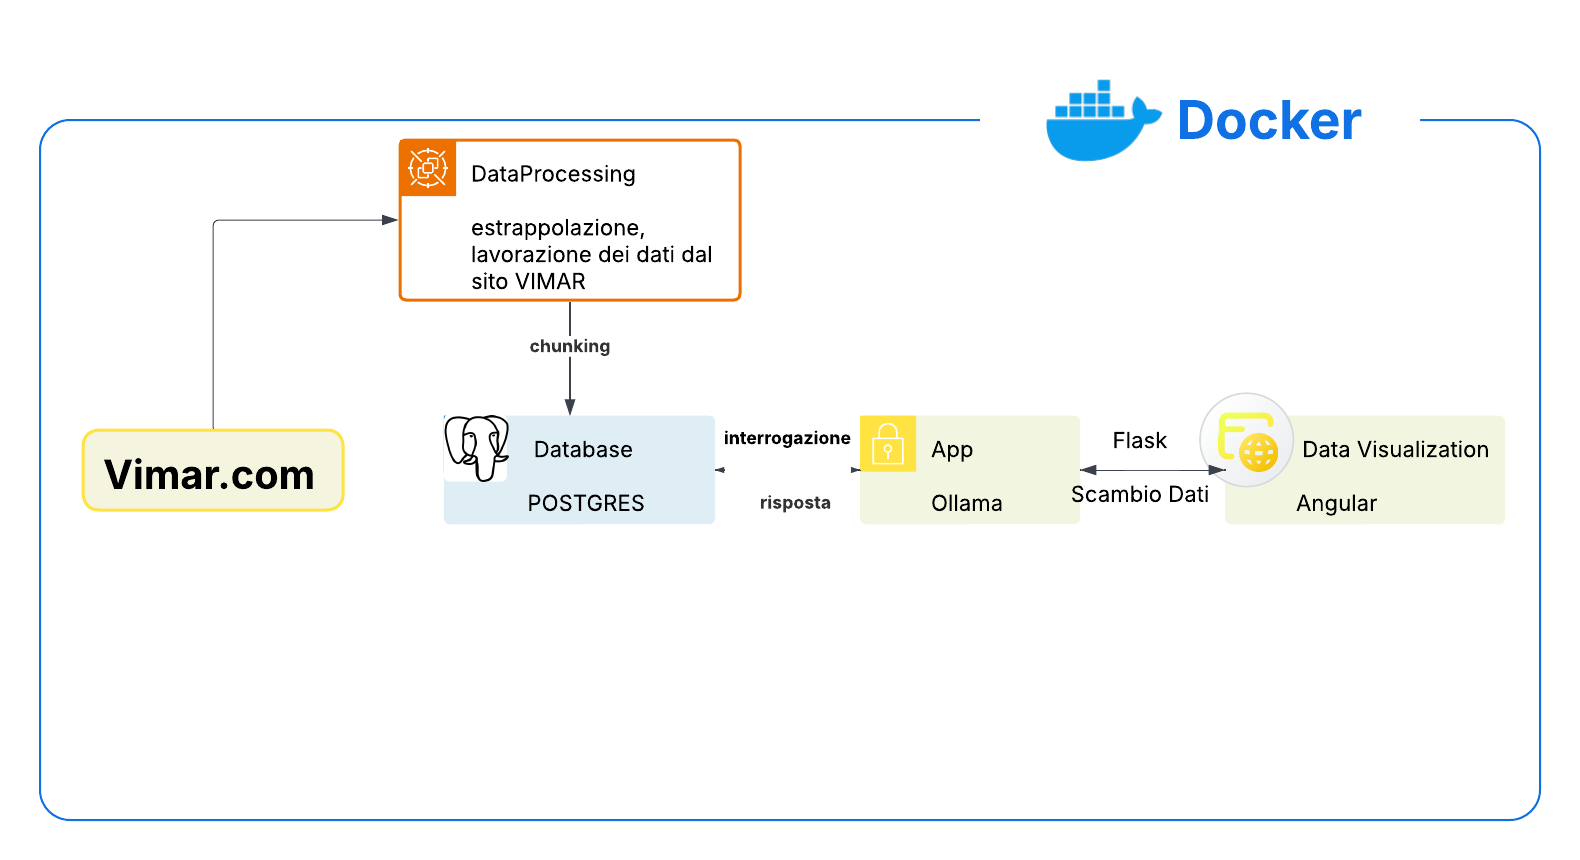
\includegraphics[width=1\textwidth]{Esagonale.png}
\end{figure}
\newpage
\section{Architettura delle compomenenti }
\end{document}
